%%%%%%%%%%%%%%%%%%%%%%%%%%%%%%% beamer %%%%%%%%%%%%%%%%%%%%%%%%%%%%%%%%%%%%%%%%%%%%%%%%%
% To run - pdflatex filename.tex
%      acroread filename.pdf
%%%%%%%%%%%%%%%%%%%%%%%%%%%%%%%%%%%%%%%%%%%%%%%%%%%%%%%%%%%%%%%%%%%%%%%%%%%%%%%%%%%%%%%%

\documentclass[compress,oilve]{beamer}
\mode<presentation>

\usetheme[]{CambridgeUS}
% other themes: AnnArbor, Antibes, Bergen, Berkeley, Berlin, Boadilla, boxes, CambridgeUS, Copenhagen, Darmstadt, default, Dresden, Frankfurt, Goettingen,
% Hannover, Ilmenau, JuanLesPins, Luebeck, Madrid, Maloe, Marburg, Montpellier, PaloAlto, Pittsburg, Rochester, Singapore, Szeged, classic

\usecolortheme{beaver}
% color themes: albatross, beaver, beetle, crane, default, dolphin,  fly, lily, orchid, rose, seagull, seahorse, sidebartab, whale, wolverine

\usefonttheme{professionalfonts}
% font themes: default, professionalfonts, serif, structurebold, structureitalicserif, structuresmallcapsserif



\hypersetup{pdfpagemode=FullScreen} % makes your presentation go automatically to full screen

% define your own colors:
\definecolor{Red}{rgb}{1,0,0}
\definecolor{Blue}{rgb}{0,0,1}
\definecolor{Green}{rgb}{0,1,0}
\definecolor{magenta}{rgb}{1,0,.6}
\definecolor{lightblue}{rgb}{0,.5,1}
\definecolor{lightpurple}{rgb}{0.8, 0.6, 0.9}
\definecolor{gold}{rgb}{.6,.5,0}
\definecolor{orange}{rgb}{1,0.4,0}
\definecolor{hotpink}{rgb}{1,0,0.5}
\definecolor{newcolor2}{rgb}{.5,.3,.5}
\definecolor{newcolor}{rgb}{0,.3,1}
\definecolor{newcolor3}{rgb}{1,0,.35}
\definecolor{darkgreen1}{rgb}{0, .35, 0}
\definecolor{darkgreen}{rgb}{0, .6, 0}
\definecolor{darkred}{rgb}{.75,0,0}
\definecolor{skyblue}{HTML}{75bbfd}

\definecolor{olive}{cmyk}{0.64,0,0.95,0.4}
\definecolor{purpleish}{cmyk}{0.75,0.75,0,0}

% can also choose different themes for the "inside" and "outside"

% \usepackage{beamerinnertheme_______}
% inner themes include circles, default, inmargin, rectangles, rounded

% \usepackage{beamerouterthemesmoothbars}
% outer themes include default, infolines, miniframes, shadow, sidebar, smoothbars, smoothtree, split, tree


\useoutertheme[subsection=true, height=40pt]{smoothbars}

% to have the same footer on all slides
%\setbeamertemplate{footline}[text line]{STUFF HERE!}
\setbeamertemplate{footline}[text line]{} % makes the footer EMPTY
% include packages
%

%show the page numbers in footnote
%\addtobeamertemplate{navigation symbols}{}{%
%	\usebeamerfont{footline}%
%	\usebeamercolor[fg]{footline}%
%	\hspace{1em}%
%	\insertframenumber/\inserttotalframenumber
%}

\setbeamercolor{footline}{fg=purpleish}
\setbeamerfont{footline}{series=\bfseries}

%add color to curent subsection
\setbeamertemplate{section in head/foot}{\hfill\tikz\node[rectangle, fill=darkred, rounded corners=1pt,inner sep=1pt,] {\textcolor{white}{\insertsectionhead}};}
\setbeamertemplate{section in head/foot shaded}{\textcolor{darkred}{\hfill\insertsectionhead}}

% Remove bullet of subsections
\setbeamertemplate{headline}
{%
	\begin{beamercolorbox}{section in head/foot}
		\insertsectionnavigationhorizontal{\textwidth}{}{}
	\end{beamercolorbox}%
}


% modify headlline, specially headline size
\setbeamertemplate{headline}{%
	\leavevmode%
	\hbox{%
		\begin{beamercolorbox}[wd=\paperwidth,ht=3.5ex,dp=1.125ex]{palette quaternary}%
			\insertsectionnavigationhorizontal{\paperwidth}{}{\hskip0pt plus1filll}
		\end{beamercolorbox}%
	}
}

\setbeamertemplate{footline}{%
	\leavevmode%
	\hbox{\begin{beamercolorbox}[wd=.5\paperwidth,ht=2.5ex,dp=1.125ex,leftskip=.3cm plus1fill,rightskip=.3cm]{author in head/foot}%
			\usebeamerfont{author in head/foot}\insertshortauthor ~ \insertshortinstitute
		\end{beamercolorbox}%
		\begin{beamercolorbox}[wd=.5\paperwidth,ht=2.5ex,dp=1.125ex,leftskip=.3cm,rightskip=.3cm plus1fil]{title in head/foot}%
			\usebeamerfont{title in head/foot}\insertshorttitle\hfill\insertframenumber\,/\,\inserttotalframenumber
	\end{beamercolorbox}}%
	\vskip0pt%
}


%\setbeamertemplate{navigation symbols}{}

\title{Chapter 4: ML Models for Tabular Datasets}
\author{ML Instruction Team, Fall 2022}
\institute[]{CE Department \newline  Sharif University of Technology \newline \newline}
\date[\today]{}
%\titlegraphic{\includegraphics[scale=.35]{example-image}}



%Write \usepackage{etex} just after the \documentclass line (it should be the first loaded package).
\usepackage{etex}
\usepackage{subcaption}
\usepackage{multicol}
\usepackage{amsmath}
\usepackage{epsfig}
\usepackage{graphicx}
\graphicspath{ {./figs/} }
\usepackage[all,knot]{xy}
\xyoption{arc}
\usepackage{url}
\usepackage{multimedia}
\usepackage{hyperref}
\hypersetup{colorlinks,linkcolor=blue,citecolor=orange,urlcolor=darkred}
\usepackage{multirow}
\usepackage[font={scriptsize}]{caption}
\usepackage{pgf}
\usepackage{fontspec}
%\setsansfont[Scale=MatchLowercase, BoldFont = * Bold, ItalicFont = * Italic]{Caladea}

\usepackage[backend=biber]{biblatex}
\addbibresource{Template-ML-Fall-200.bib}
%\usepackage{enumitem,xcolor}
%\newcommand{\labelitemi}{$\blacksquare$}
%\newcommand{\labelitemii}{$\diamond$}
%\newcommand{\labelitemiii}{$\square$}
%\newcommand{\labelitemiv}{$\ast$}
%\setbeamercolor*{item}{fg=red}



\usefonttheme{professionalfonts} 
\setbeamertemplate{itemize item}{\color{skyblue}$\blacksquare$}
\setbeamertemplate{itemize subitem}{\color{hotpink}$\blacktriangleright$}
\setbeamertemplate{itemize subsubitem}{\color{orange}$\bullet$}


\usepackage{anyfontsize}
\usepackage{t1enc}
\usepackage{tikz}
\usetikzlibrary{calc,trees,positioning,arrows,chains,shapes.geometric,decorations.pathreplacing,decorations.pathmorphing,shapes,matrix,shapes.symbols}



\newtheorem{proposition}[theorem]{Proposition}
\newtheorem{remark}[theorem]{Remark}
\newtheorem{assumption}[theorem]{Assumption}

\usepackage{xcolor}
% \newcommand{\tc}[2]{
% 	\textcolor{#1}{#2}
% }
\newcommand{\tc}[2]{
 \textcolor{#1}{\tc{keywords}{#2}}
}

%\usepackage{fontspec, unicode-math}
%\setmainfont[Scale=0.9]{Nimbus Roman No9 L}
%\setmonofont[Scale=0.9]{Monaco}
\setsansfont[Scale=1]{Times New Roman}

\newcommand{\vect}[1]{\boldsymbol{#1}}

\definecolor{strings}{rgb}{.624,.251,.259}
\definecolor{keywords}{rgb}{.224,.451,.686}
\definecolor{comment}{rgb}{.322,.451,.322}


%\usepackage{smartdiagram}
%\usesmartdiagramlibrary{additions}
%%%%%%%%%%%%%%%%%%%%%%%%%%%%%%%%%%%%%%%%%%%%%%%%%%%%%%%%%%%%%%%%%%%%%%%%%%%%%%%%%%%%%%%%%%%%
%%%%%%%%%%%%%%%%%%%%%%%%%%%%%% Title Page Info %%%%%%%%%%%%%%%%%%%%%%%%%%%%%%%%%%%%%%%%%%%
%%%%%%%%%%%%%%%%%%%%%%%%%%%%%%%%%%%%%%%%%%%%%%%%%%%%%%%%%%%%%%%%%%%%%%%%%%%%%%%%%%%%%%%%%%


%%%%%%%%%%%%%%%%%%%%%%%%%%%%%%%%%%%%%%%%%%%%%%%%%%%%%%%%%%%%%%%%%%%%%%%%%%%%%%%%%%%%%%%%%%
%%%%%%%%%%%%%%%%%%%%%%%%%%%%%% Begin Your Document %%%%%%%%%%%%%%%%%%%%%%%%%%%%%%%%%%%%%%%
%%%%%%%%%%%%%%%%%%%%%%%%%%%%%%%%%%%%%%%%%%%%%%%%%%%%%%%%%%%%%%%%%%%%%%%%%%%%%%%%%%%%%%%%%%
\begin{document}
	
%%%%%%%%%%%%%%%%%%%%%%%%%%%%%%%%%%%%%%%%%%%%%%%%%%%%%%%%%%%%%%%%%%%%%%%%%%%%%%%%%%%%%%%%%%
	\fontsize{9}{9}
\begin{frame}[noframenumbering, plain]
	\titlepage
\end{frame}

%%%%%%%%%%%%%%%%%%%%%%%%%%%%%%%%%%%%%%%%%%%%%%%%%%%%%%%%%%%%%%%%%%%%%%%%%%%%%%%%%%%%%%%%%%
\section{Ensemble methods}
%%%%%%%%%%%%%%%%%%%%%%%%%%%%%%%%%%%%%%%%%%%%%%%%%%%%%%%%%%%%%%%%%%%%%%%%######
\frame{\frametitle{Ensemble methods}
\begin{itemize}
	\item 
	\textbf{Ensemble methods} is a machine learning technique that combines several base models in order to produce one optimal predictive model.
    \begin{figure}[t]
    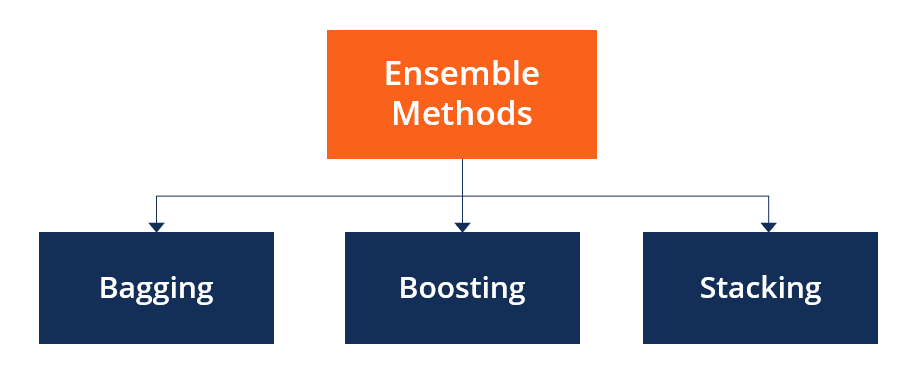
\includegraphics[scale=0.6]{EnsMeth.png}
    \caption{Three main approaches, \href{https://corporatefinanceinstitute.com/resources/knowledge/other/ensemble-methods/}{(Source)}}
    \centering
    \end{figure}
\end{itemize}
}

\frame{\frametitle{When to use Ensemble learning}
\vspace{-3cm}
\begin{itemize}
\item
Ensemble learning works best when the base models are not correlated. Models with high correlation tend to deviate towards same direction, thus, promediating a greater and more correlated error.
\medskip
\item
It also helps with reducing variance and making more robust models. More samples lead to more unbiased predictor. (Due to Central limit theorem)
\medskip
\item
You will often use Ensemble methods \textbf{near the end of a project} , once you have already built a few good predictors, to combine them into an even better predictor.

\end{itemize}
}

\section{Voting Classifiers}
%%%%%%%%%%%%%%%%%%%%%%%%%%%%%%%%%%%%%%%%%%%%%%%%%%%%%%%%%%%%%%%%%%%%%%%%%%%%%%%%%%%%%%%%%%%%%%%
\frame{\frametitle{Hard Voting}
\begin{itemize}
	\item 
	\textbf{Hard Voting} $\rightarrow$    Majority Vote
	%Hands-On Machine Learning with Scikit-Learn and TensorFlow, Chapter 7
	\begin{figure}[t]
	
    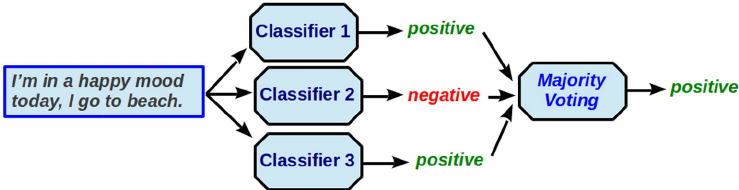
\includegraphics[scale=0.4]{Hard-Voting.png}
    \centering
    \caption{Example of Majority Voting, \href{https://www.researchgate.net/figure/An-example-of-majority-voting-as-the-combination-rule-In-this-case-the-majority-of-the_fig2_264242096}{(Source)}}
    \end{figure}
$$\hat{y} = arg \max\limits_j \sum_{i=1}^{n} h_i^j(x)$$
$$H(x) = \{h_1,h_2, ..., h_n\}, h_i^j(x) \in [0,1]$$
$h_i^j(x)$: The predicted class membership probability of the $i$th classifier for
class label $j$.
\end{itemize}	
}

\frame{\frametitle{Why Majority Voting?}
\begin{itemize}
\item
Assume $n$ independent (errors are uncorrelated) binary classifiers with a base error rate $\epsilon$. (better than random guessing)
\medskip
\item
Probability of making a wrong prediction via the ensemble if $k$ classifiers predict same class label:
$$P(k) = \binom{n}{k}\epsilon^k(1 - \epsilon)^{n-k}, k > \lceil n/2 \rceil$$
\item
\textbf{Ensemble error:}
$$\epsilon_{ens} = \sum_{k}^{n} \epsilon^k(1 - \epsilon)^{n-k}, k > \lceil n/2 \rceil$$
\begin{figure}[t]
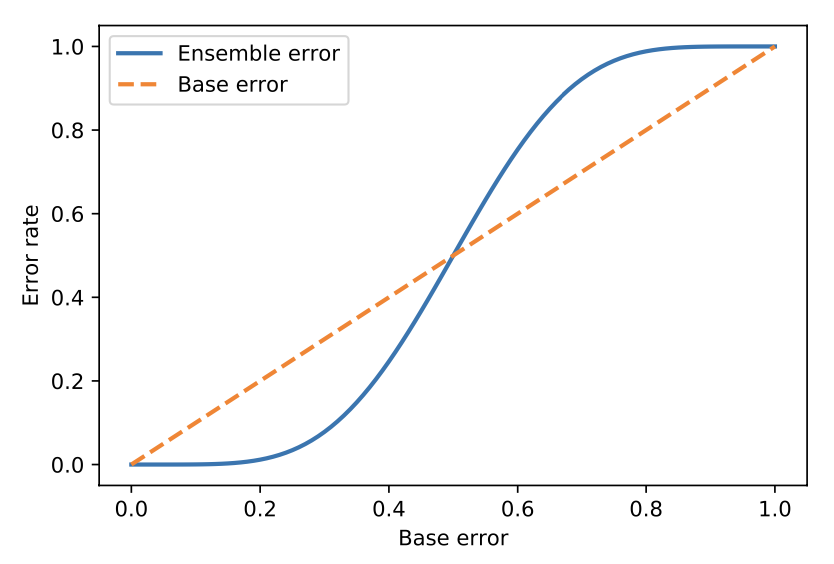
\includegraphics[scale=0.3]{ErrorRate.png}
\caption{Ensemble error plot\cite{slides}}
\centering
\end{figure}
\end{itemize}
}


\frame{\frametitle{Soft Voting}

\begin{itemize}
	\item 
	\textbf{Soft Voting} $\rightarrow$   Highest class probability (When \textbf{all} classifiers are able to estimate class probabilities)
		
	\begin{figure}[t]
    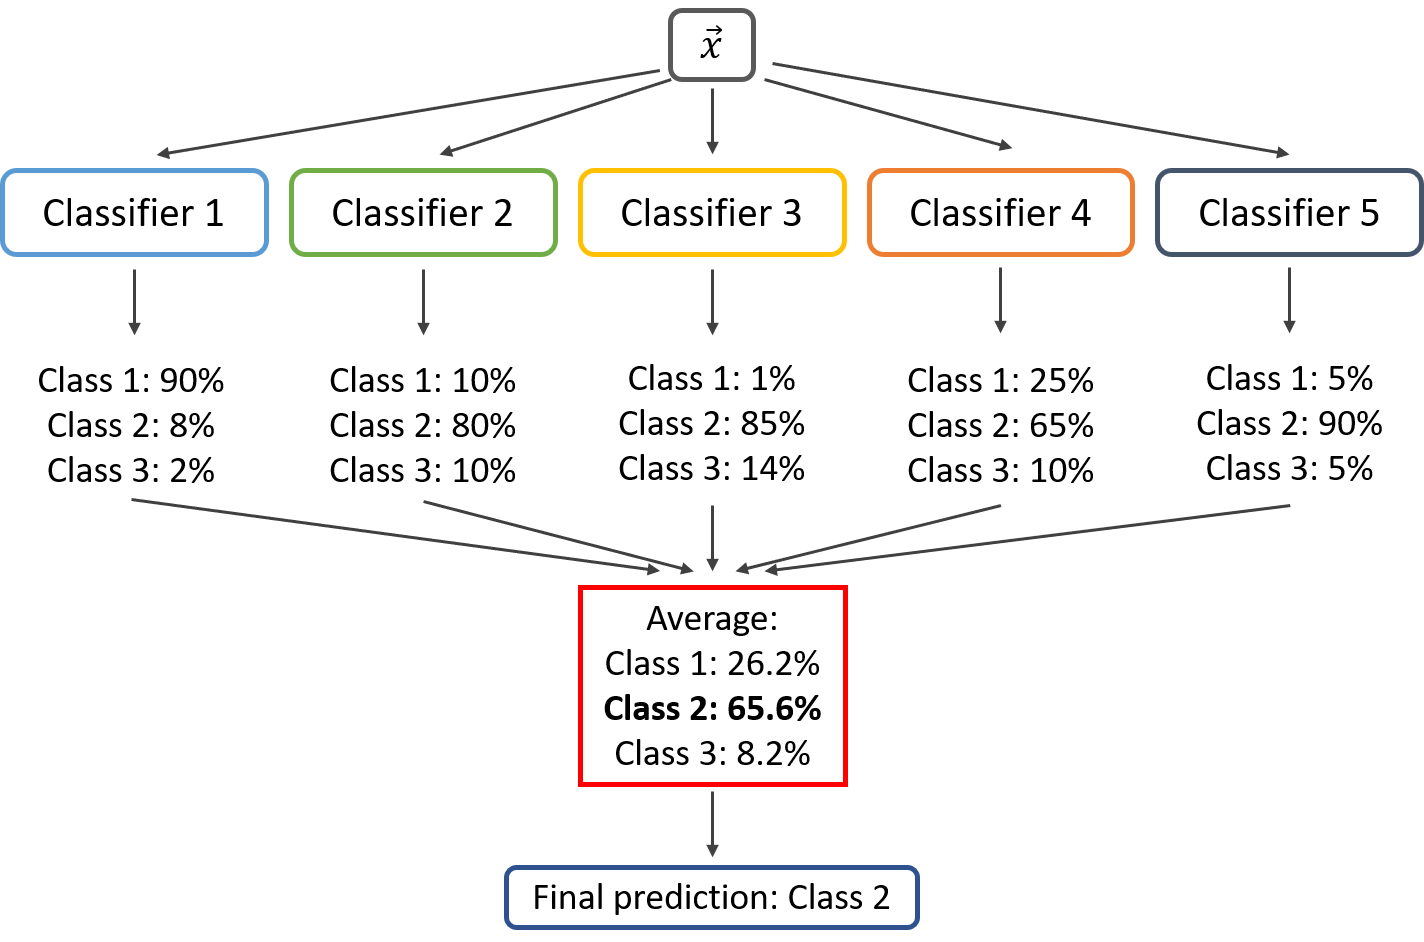
\includegraphics[scale=0.18]{Soft-Voting.png}
    \caption{Example of Soft Voting, \href{https://iq.opengenus.org/voting-classifier/}{(Source)}}
    \centering
    \end{figure}
\end{itemize}
}

\frame{\frametitle{Soft Voting}

$$\hat{y} = arg \max\limits_j \sum_{i=1}^{n} w_i h_i^j(x), w_i > 0, \sum_{i=1}^{n} w_i = 1$$
$$H(x) = \{h_1,h_2, ..., h_n\}, h_i^j(x) \in [0,1]$$
\begin{itemize}
\item
$h_i^j(x)$: The predicted class membership probability of the $i$th classifier for
class label $j$, $w_i$ is the optional weighting parameter. \textbf{Example:}
\end{itemize}
\begin{figure}[t]
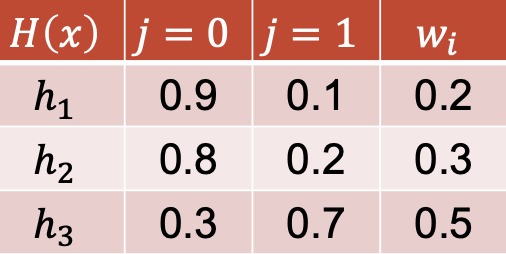
\includegraphics[scale=0.3]{SoftVotingEX.png}
\caption{Probability and Weights of each predictor\cite{awesome}}
\centering
\end{figure}
$$p(j=0|x) = 0.2*0.9 + 0.3*0.8 + 0.3*0.5 = 0.57$$
$$p(j=1|x) = 0.2*0.1 + 0.3*0.2 + 0.3*0.7 = 0.28$$
$$\hat{y} = arg \max\limits_j{p(j=0|x), p(j=1|x)} = 0 $$
}

\frame{\frametitle{Plurality Voting}
\vspace{-2cm}
\begin{itemize}
\item 
	\textbf{Plurality Voting (Unstable)} $\rightarrow$   Most Voted (When none of the predictions get more than half of the votes)
	\bigskip
	\begin{figure}[t]
    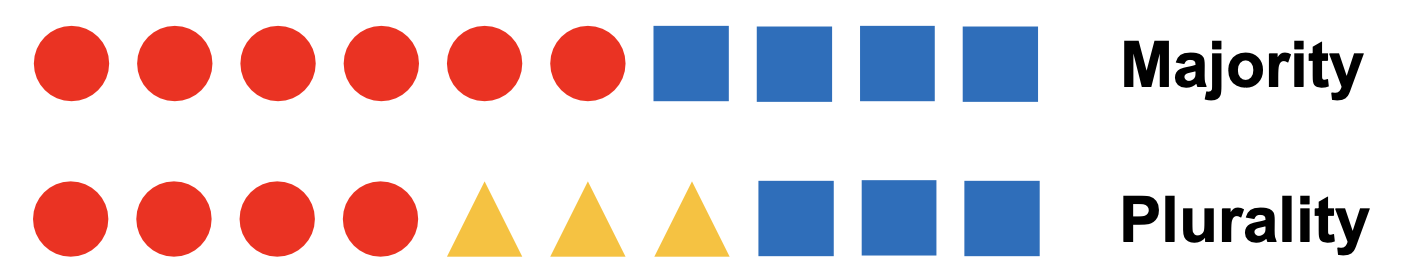
\includegraphics[scale=0.45]{MajPlu.png}
    \caption{Majority vs Plurality\cite{awesome}}
    \centering
    \end{figure}
\end{itemize}
}



\section{Bagging}
%%%%%%%%%%%%%%%%%%%%%%%%%%%%%%%%%%%%%%%%%%%%%%%%%%%%%%%%%%%%%%%%%%%%%%%%%%%%%%%%%%%%%%%%%%%%%%%
\frame{\frametitle{Bootstrapping}
\vspace{-1cm}
\begin{itemize}
\item
A resample method that consists of repeatedly drawn, with replacement, samples from data to form other smaller datasets. (The observations \textbf{can} appear more than one time)

\begin{figure}[t]
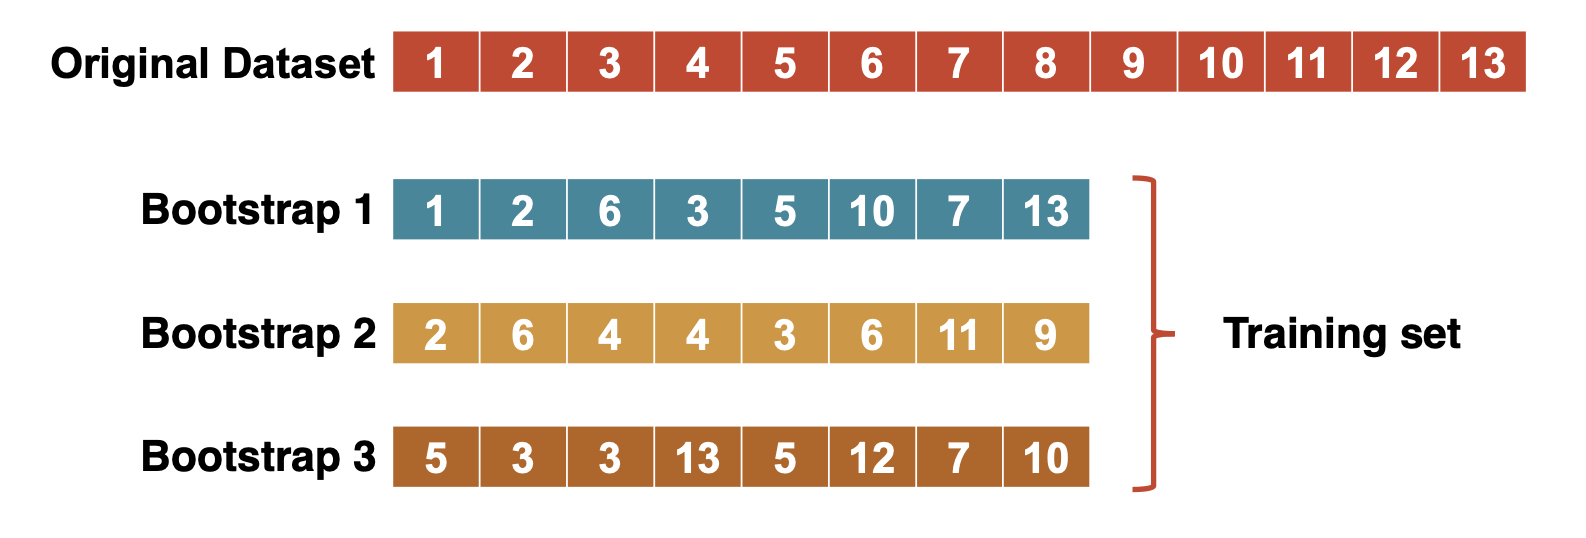
\includegraphics[scale=0.4]{Bootstrap2.png}
\caption{Example of Bootstrapping\cite{awesome}}
\end{figure}
\end{itemize}
}

\frame{\frametitle{Bagging}
\vspace{-1cm}
\begin{itemize}
	\item 
	Use the same algorithm for every predictor and train them on different random subsets.
    \begin{itemize}
	\item 
	Sampling with replacement: \textbf{Bagging} (Bootstrap Aggregating)
	\item
	Sampling without replacement: \textbf{Pasting}
	\end{itemize}
	\item
    In this approach we generate $B$ different bootstrapped training data sets.
    $$\hat{f}_{bag}(x) = \frac{1}{B}\sum_{b=1}^{B}\hat{f}^{*b}(x)$$
    \item
    The aggregation function is typically:
        \begin{itemize}
            \item 
            Mode (Most frequent) for Classification
            \item
            Average for Regression
        \end{itemize}
    \smallskip
    \item
    Predictors can all be trained in parallel, via different CPU cores or even different servers. Similarly, predictions can be made in parallel.
\end{itemize}	
}

\frame{\frametitle{Bagging}
\begin{figure}[t]
    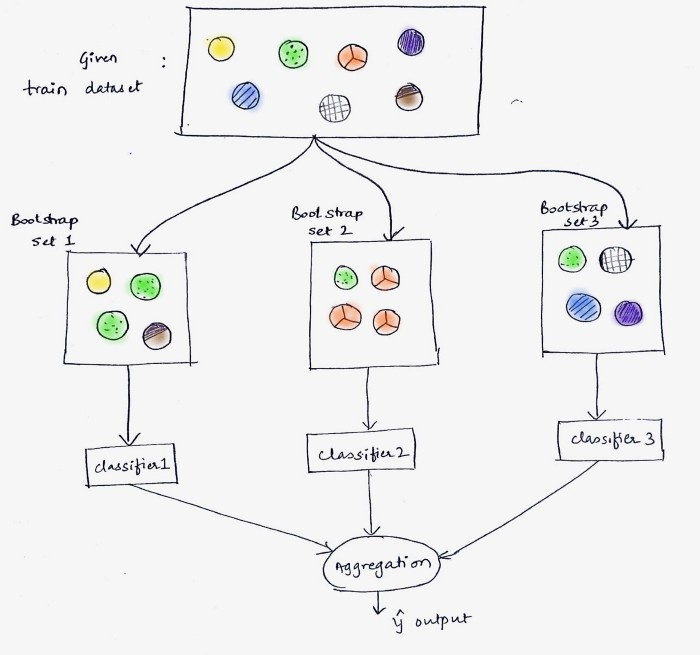
\includegraphics[scale=0.3]{Bagging.jpeg}
    \caption{Example of Bagging, \href{https://medium.com/machine-learning-through-visuals/machine-learning-through-visuals-part-1-what-is-bagging-ensemble-learning-432059568cc8}{(Source)}}
    \centering
\end{figure}
}


% \frame{\frametitle{Bias and Variance}
% \begin{figure}[t]
%     \includegraphics[scale=0.3]{BV.png}
%     \centering
% \end{figure}
% }

% \frame{\frametitle{Bagging effect on Bias and Variance}

% \begin{itemize}
% \item
% Each individual predictor has a higher bias than if it were trained on the original training set, but aggregation reduces both bias and variance. 
% \begin{figure}[t]
%     \includegraphics[scale=0.45]{DTBV.png}
%     \centering
% \end{figure}
% \item
% Bootstrapping introduces a bit more diversity in the subsets that each predictor is trained on, so bagging ends up with a slightly higher bias than pasting.
% \end{itemize}
% }





\frame{\frametitle{Out-of-Bag Evaluation}
\vspace{-2cm}
\begin{itemize}
\item
With bagging, some instances may be sampled several times for any given predictor, while others may not be sampled at all. 
\smallskip
\item
The remaining of the training instances that are not sampled are called \textbf{out-of-bag (OOB)} instances.
$$P(NotChosen) = (1 - \frac{1}{n})^n, n \to \infty$$
$$ \frac{1}{e} \approx 0.368$$
$$P(Chosen) = 1 - (1 - \frac{1}{n})^n \approx 0.632$$
\item
This means that when the dataset is big enough, \textbf{37\%} of its samples are never selected and we could use it to test our model.
\end{itemize}
}

\frame{\frametitle{$P(Chosen)$}

\begin{figure}[t]
    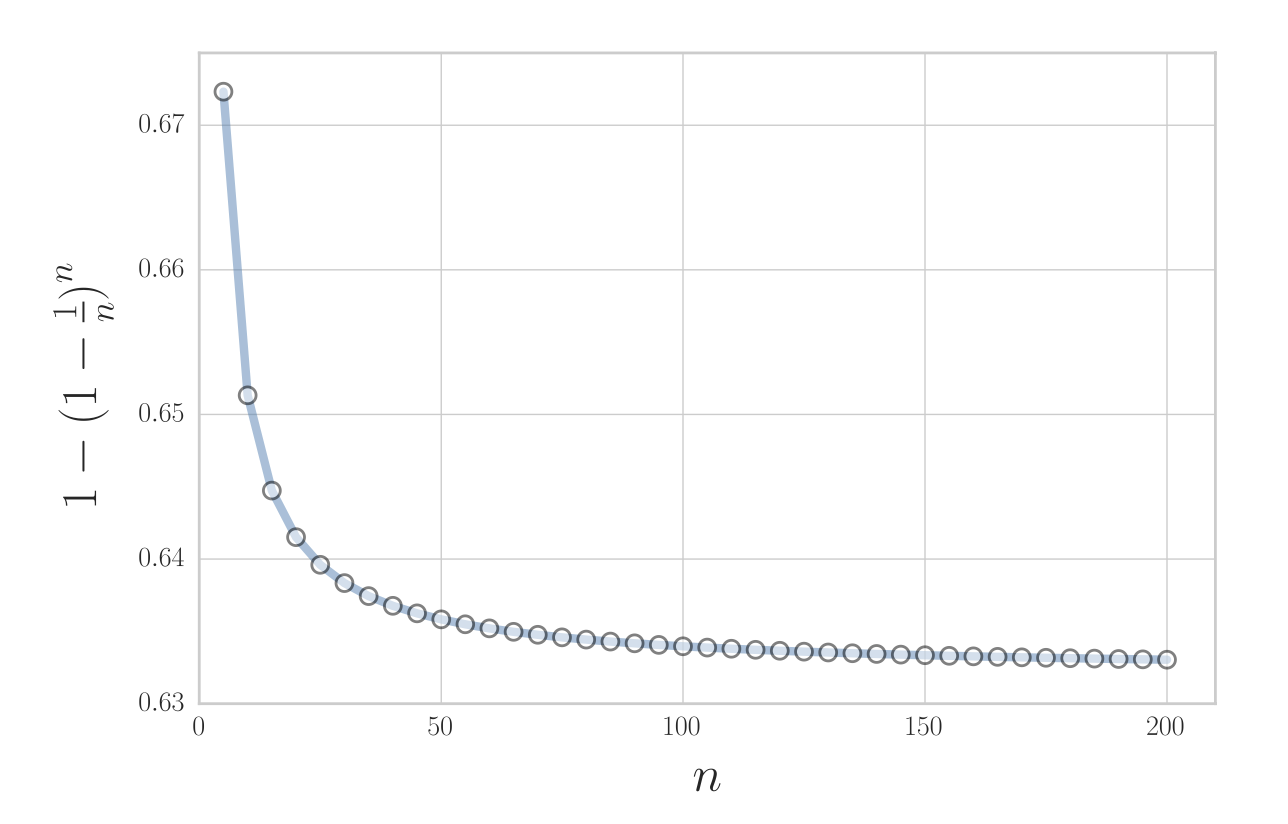
\includegraphics[scale=0.45]{Chosen.png}
    \caption{Plot of $P(Chosen)$\cite{notes}}
    \centering
\end{figure}
}

\frame{\frametitle{Random Patches and Random Subspaces}
\vspace{-3cm}
\begin{itemize}
\item
You can sample \textbf{features} instead of instances and train each predictor on them.
\begin{itemize}
\item
Sampling both training instances and features is called the \textbf{Random Patches} method.
\item
But keeping all training instances, but sampling features is called the \textbf{Random Subspaces} method.
\end{itemize}
\medskip
\item
They are useful when you are dealing with high-dimensional inputs. (such as images)
\medskip
\item
Sampling features leads to trading a bit more bias for a lower variance.
\end{itemize}
}


\section{Random Forests}
%%%%%%%%%%%%%%%%%%%%%%%%%%%%%%%%%%%%%%%%%%%%%%%%%%%%%%%%%%%%%%%%%%%%%%%%%%%%%%%%%%%%%%%%%%%%%%%
\frame{\frametitle{Random Forests}

\begin{itemize}
\item
\textbf{Ensemble of Decision Trees}. Generally uses bagging and feature randomness to try to create an uncorrelated forest of trees.
\item
Instead of searching for the very best feature when splitting a node, it searches for the best feature among a \textbf{random subset of features}.
\begin{figure}[t]
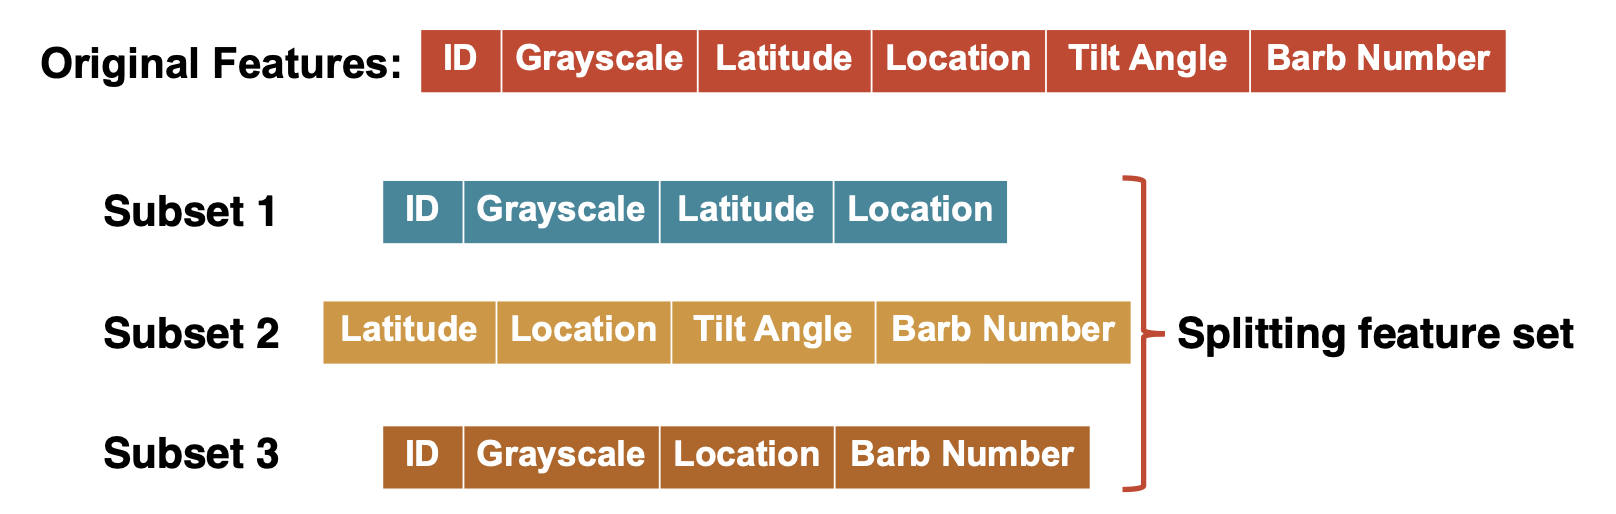
\includegraphics[scale=0.35]{RFsub.png}
\caption{Split based on features\cite{awesome}}
\centering
\end{figure}
\item
It is possible to make trees even more random by also using random thresholds for each feature rather than searching for the best possible thresholds.
\item
It is called an \textbf{Extremely Randomized Trees ensemble} or \textbf{Extra-Trees} for short.
\end{itemize}	
}

\frame{\frametitle{Steps of Random Forest}

\begin{figure}[t]
    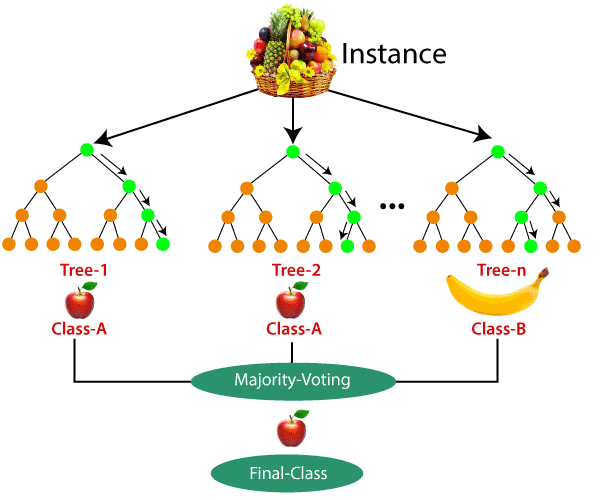
\includegraphics[scale=0.35]{RFstep.png}
    \caption{Example of Random forest, \href{https://www.section.io/engineering-education/introduction-to-random-forest-in-machine-learning/}{(Source)}}
    \centering
\end{figure}
}


\frame{\frametitle{Features of Random Forest}
\vspace{-2cm}
\begin{itemize}
\item
Pros:
    \begin{itemize}
    \item
    It can be used for both regression and classification tasks
    \item
    Higher accuracy
    \item
    Reduce risk of overfitting
    \item
    Measures feature’s importance
    \end{itemize}
\item
Cons:
    \begin{itemize}
    \item
    Time consuming (ineffective for real-time predictions)
    \item
    Many parameters: depth of tree, number of trees, type of node tests, random sampling
    \item
    Requires a lot of training data and large memory footprint
    \item
    Sacrifice the interpretability of model
    \end{itemize}
\end{itemize}
}


\section{Boosting}
%%%%%%%%%%%%%%%%%%%%%%%%%%%%%%%%%%%%%%%%%%%%%%%%%%%%%%%%%%%%%%%%%%%%%%%%%%%%%%%%%%%%%%%%%%%%%%%
\frame{\frametitle{Boosting}
\vspace{-2cm}
\begin{itemize}
    \item 
    \textbf{Boosting} (originally called hypothesis boosting) refers to any Ensemble method that can combine several weak learners into a strong learner.
    \item
    The model is weak if it has a substantial error rate, but the performance is not random.
    \medskip
    \item
    The general idea of most boosting methods is to train predictors sequentially, each trying to correct its predecessor.
    \item 
    Most popular boosting methods (Differ in terms of how weights are updated 
    \& classifiers are combined):
    \begin{itemize}
        \item 
        Adaptive Boosting (AdaBoost)
        \item
        Gradient Boosting (LightGBM, XGBoost)
    \end{itemize}
\end{itemize}
}

\frame{\frametitle{Boosting}
    \begin{figure}[t]
    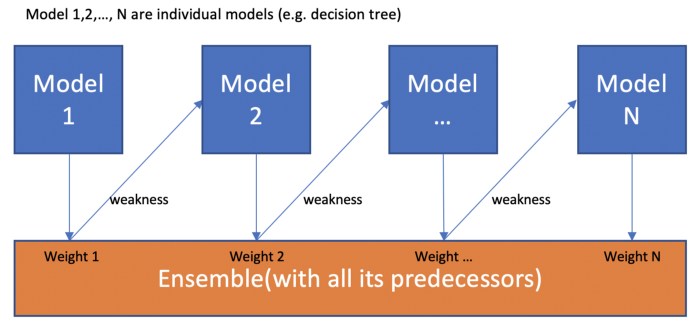
\includegraphics[scale=0.5]{Boosting.png}
    \caption{Boosting Process, \href{https://towardsdatascience.com/boosting-algorithms-explained-d38f56ef3f30}{(Source)}}
    \centering
    \end{figure}

}


\frame{\frametitle{AdaBoost}

\begin{itemize}
\item
One way for a new predictor to correct its predecessor is to pay a bit more attention to the training instances that the predecessor underfitted.
\item
This results in new predictors focusing more and more on the hard cases.

% \begin{figure}[t]
%     \includegraphics[scale=0.35]{AdaBoost.png}
%     \centering
% \end{figure}

\item
\textbf{Drawback of AdaBoost}: It doesn't scale as well as bagging (or pasting). 
\end{itemize}
}

\frame{\frametitle{AdaBoost Steps}

\begin{itemize}
    \item 
    First trains a base classifier and uses it to make predictions
    \item
    Then increases the relative weight of misclassified instances
    \item
    Then it trains a second classifier, using the updated weights, and again makes predictions and so on...
\begin{figure}[t]
    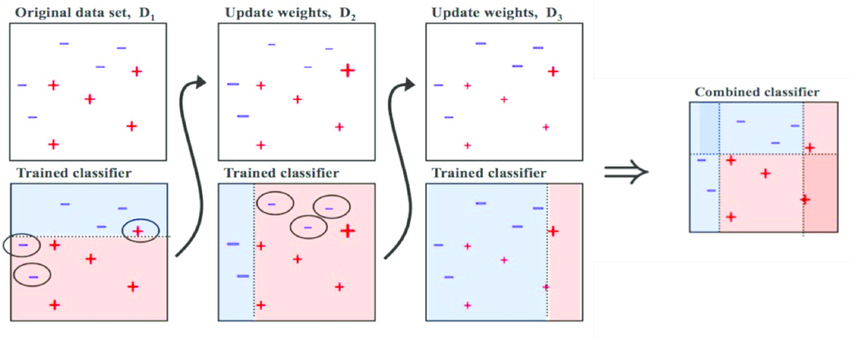
\includegraphics[scale=0.3]{BoostIter.png}
    \caption{AdaBoost Steps, \href{https://iq.opengenus.org/types-of-boosting-algorithms/}{(Source)}}
    \centering
\end{figure}
    \item
    Once all predictors are trained, the ensemble makes predictions very much like bagging, except that predictors have different weights.
\end{itemize}
}

\frame{\frametitle{AdaBoost Algorithm}

\begin{itemize}
\item
Each instance weight $w^{(i)}$ is initially set to $1/m$ and first predictor's weighted error rate is $r_1$.

\item
Weighted error rate of the $j^{th}$ predictor:
$$r_j = \frac{\sum\limits_{\substack{i=1 \\ \hat{y}_j^{(i)} \neq y^{(i)}  }}^m w^{(i)}}{\sum_{i=1}^{m} w^{(i)}}$$
where $\hat{y}_j^{(i)}$ is the $j^{th}$ predictor's prediction for the $i^{th}$ instance.

\item
The predictor's weight:
$$\alpha_j = \eta \log \frac{1 - r_j}{r_j}$$
where $\eta$ is the learning rate. 
\begin{itemize}
    \item 
    The more accurate the predictor is, the higher its weight will be. 
    \item
    If it is just guessing randomly, then its weight will be close to zero. 
    \item
    However, if it is most often wrong, then its weight will be negative.
\end{itemize}
\end{itemize}
}


\frame{\frametitle{AdaBoost Algorithm}
\vspace{-1cm}
\begin{itemize}
\item
Next, the AdaBoost algorithm update the instance weights, which boosts the weights of the misclassified instance:
$$w^{(i)} \gets
\begin{cases}
  w^{(i)}  & \text{if } \hat{y}_j^{(i)} = y^{(i)} \\
  w^{(i)} \exp(\alpha_j) & \text{if } \hat{y}_j^{(i)} \neq y^{(i)}
\end{cases}$$
Then all the instance weights gets normalized by dividing by $\sum_{i=1}^{m} w^{(i)}$.

\item
Finally, a new predictor is trained using the updated weights, and the whole process is repeated.
\item
The algorithm stops when the desired number of predictors is reached, or when a perfect predictor is found.
\item
AdaBoost predictions:
$$\hat{y}(x) =argmax \sum\limits_{\substack{j=1 \\ \hat{y}_j(x)=k}}^N \alpha_j$$

\end{itemize}
}


\frame{\frametitle{Gradient Boosting}

\begin{itemize}
\item
In this approach, instead of tweaking the instance weights at every iteration like AdaBoost does, this method tries to fit the new predictor to the residual errors made by the previous predictor.
\end{itemize}
\begin{figure}[t]
    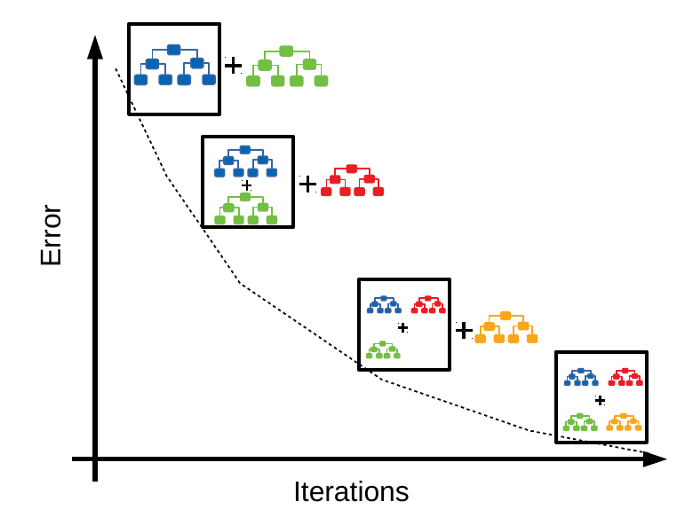
\includegraphics[scale=0.28]{GradBoost.png}
    \caption{Gradient Boosting Process, \href{https://medium.com/swlh/gradient-boosting-trees-for-classification-a-beginners-guide-596b594a14ea}{(Source)}}
    \centering
\end{figure}
}


\frame{\frametitle{Gradient Boosting Steps}

\textbf{Example:}
\begin{figure}[t]
    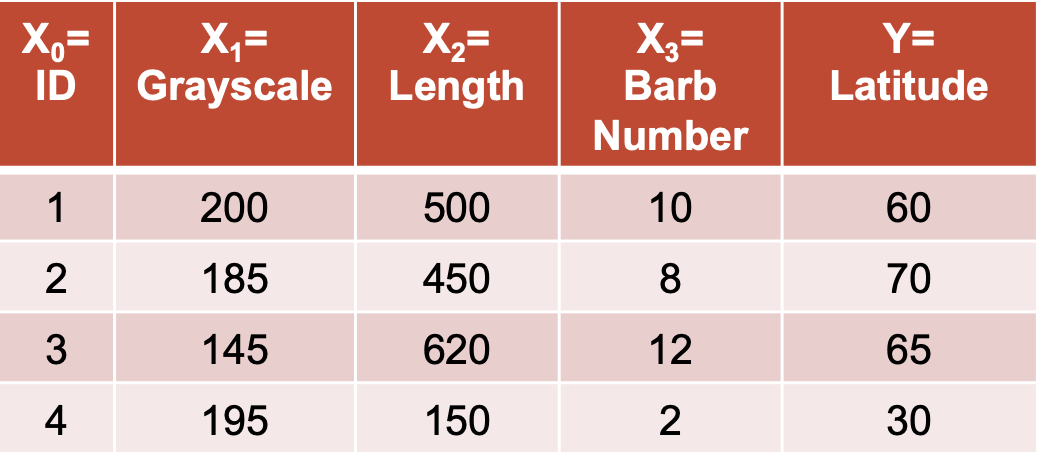
\includegraphics[scale=0.3]{GB1.png}
    \caption{Dataset\cite{awesome}}
    \centering
\end{figure}
\begin{itemize}
\item
Construct base tree(just the root node):
$$y_1^{*} = \frac{1}{n}\sum_{i=1}^{n}y^i = 56.25 $$
\end{itemize}
}

\frame{\frametitle{Gradient Boosting Steps}

\begin{itemize}
\item
Build next tree based on errors of the previous tree:
$$r_1 = y_1 - y_1^{*}$$
\end{itemize}
\begin{figure}[t]
    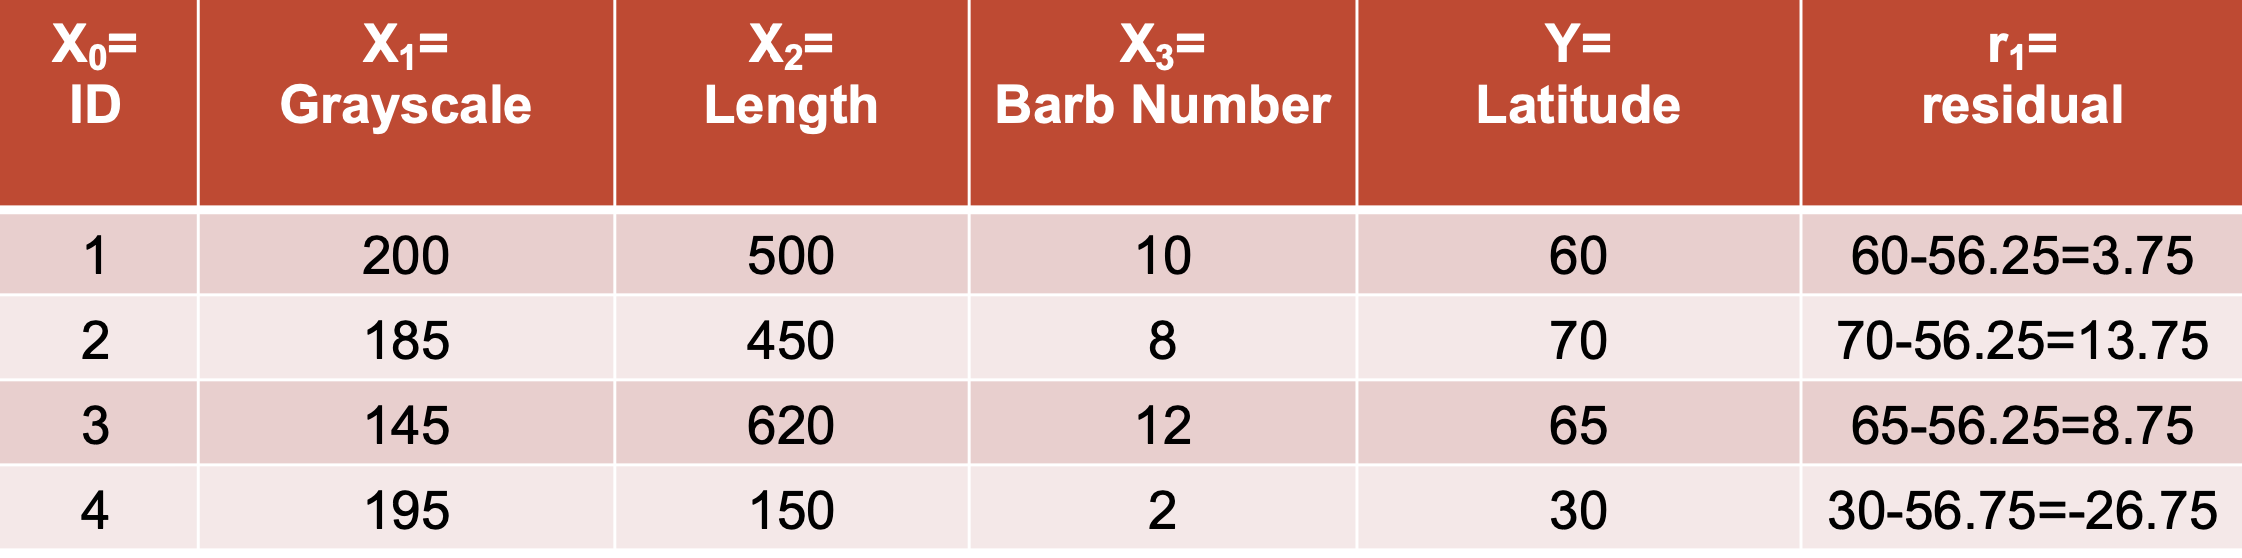
\includegraphics[scale=0.3]{GB2.png}
    \caption{Dataset after calculating residuals\cite{awesome}}
    \centering
\end{figure}
}

\frame{\frametitle{Gradient Boosting Steps}

\begin{itemize}
\item
Then, create a tree based on $x_1, x_2, ...,x_m$ to fit the residuals:
\begin{figure}[t]
    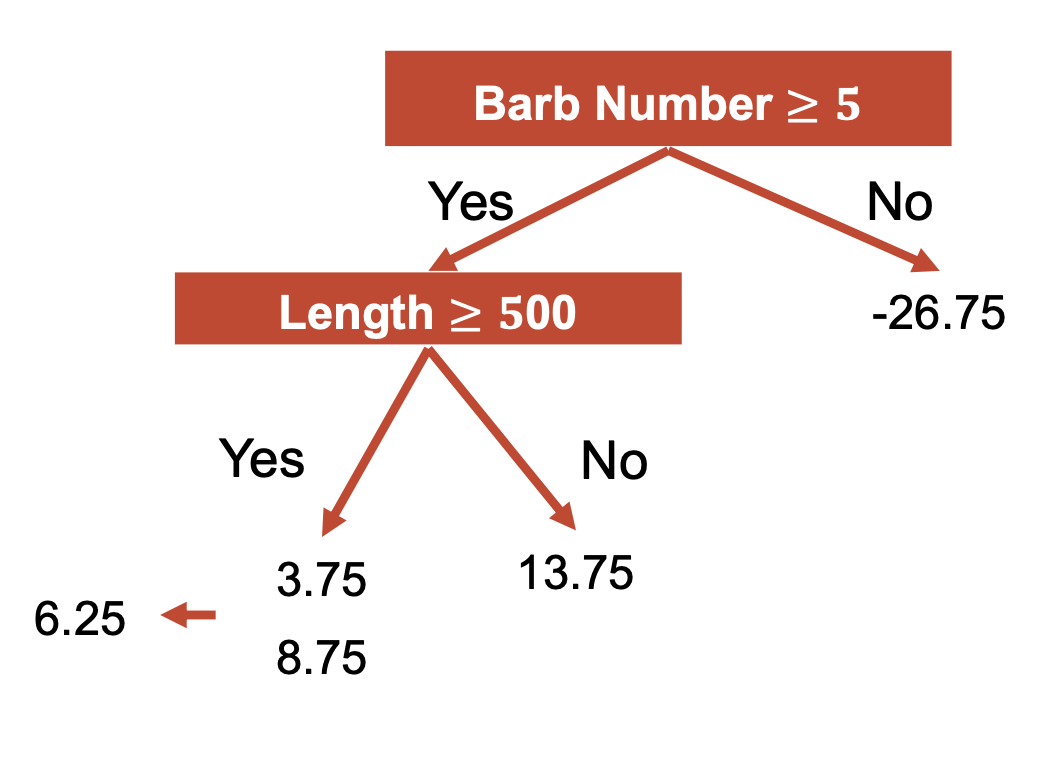
\includegraphics[scale=0.3]{GB3.png}
    \caption{Create a tree\cite{awesome}}
    \centering
\end{figure}
\item
Combine tree from step 1 with tree:
$$\text{Predict (ID=3):} 56.25 + \alpha*6.25$$
Where $\alpha$ learning rate between 0 and 1(if $\alpha = 1$, low bias but high variance)
\end{itemize}
}

% \frame{\frametitle{Gradient Boosting Algorithm}
% \begin{itemize}

% \item
% \textbf{Step 0}: Input data $\{\langle x^{(i)}, y^{(i)} \rangle   \}_{i=1}^{n}$ \\
% Differentiable Loss function $L(y^{(i)},h(x^{(i)}))$

% \item
% \textbf{Step 1}: Initialize model $h_0(x) = argmin \sum_{i=1}^{n} L(y^{(i)},\hat{y})$

% \item
% \textbf{Step 2}: for $t=1$ to $T$ (Number of trees to make)
%     \begin{itemize}
%         \item 
%         \textbf{A.} Compute pseudo residual
%         $$r_{i,t} = - [\frac{\partial L(y^{(i)}, h(x^{(i)}))}{\partial h(x^{(i)})}]$$
%         for the $t$-th tree and $i$-th example
%         \item
%         \textbf{B.} Fit tree to $r_{i,t}$ values, and create terminal nodes $R_{j,t}$ for $j=1,...,J_t$
%     \end{itemize}

% \end{itemize}
% }

% \frame{\frametitle{Gradient Boosting Algorithm}
% \begin{itemize}
%     \item 
    
%     \begin{itemize}
%         \item
%         \textbf{C.} for $j=1,...,J_t$, compute:
%         $$\hat{y}_{j,t}=argmin \sum_{x^{(i)} \in R_{i,j} } L(y^{(i)}, h_{t-1}(x^{(i)}) + \hat{y} )$$
%         \item
%         \textbf{D.} Update 
%         $$h_t(x)=h_{t-1}(x) + \alpha \sum_{j=1}^{J_t} \hat{y}_{j,t}  (x \in R_{j,t})$$
%     \end{itemize}
    
%     \item
%     \textbf{Step 3}: Return $h_t(x)$
% \end{itemize}
% }


\frame{\frametitle{XGBoost}

\begin{itemize}
\item
\textbf{XGBoost}, which stands for Extreme Gradient Boosting, is a scalable, distributed gradient-boosted decision tree (GBDT) machine learning library. 
\item
It provides parallel tree boosting and is the leading machine learning library for regression, classification, and ranking problems.
\item
The main difference is that XGBoost uses a more regularized model, which helps to prevent overfitting.
\end{itemize}
%
\begin{figure}[t]
    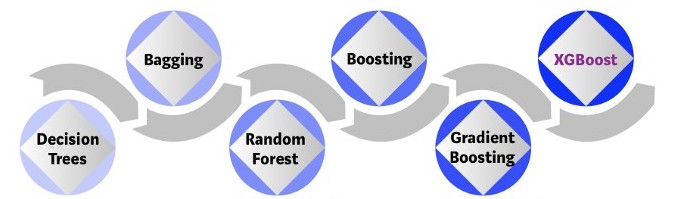
\includegraphics[scale=0.4]{Evolution.jpeg}
    \caption{Evolution of tree-based algorithms, \href{https://towardsdatascience.com/https-medium-com-vishalmorde-xgboost-algorithm-long-she-may-rein-edd9f99be63d}{(Source)}}
    \centering
\end{figure}
}

\frame{\frametitle{XGBoost}
\vspace{-2cm}
\begin{itemize}
\item
XGBoost uses pre-sorted algorithm \& Histogram-based algorithm for computing the best split.
\item
\textbf{Pre-Sorting splitting}
    \begin{itemize}
        \item For each node, enumerate over all features
        \item For each feature, sort the instances by feature value
        \item Use a linear scan to decide the best split along that feature basis information gain
        \item Take the best split solution along all the features
    \end{itemize}
\item
In simple terms, Histogram-based algorithm splits all the data points for a feature into discrete bins and uses these bins to find the split value of histogram.
\end{itemize}

}

\frame{\frametitle{CatBoost}
\begin{itemize}
    \item 
    An open-source machine learning algorithm which allows users to quickly handle categorical features for a large dataset.
    \medskip
    \item
    CatBoost uses oblivious decision trees, where the same splitting criterion is used across an entire level of the tree.
    \item
    Advantages:
    \begin{itemize}
        \item 
        No need to preprocess categorical features and also Support missing value
        \item
        No overfitting unlike Gradient Boosting
        \item
        It has all the good features of others boosting
    \end{itemize}
\end{itemize}
\begin{figure}[t]
    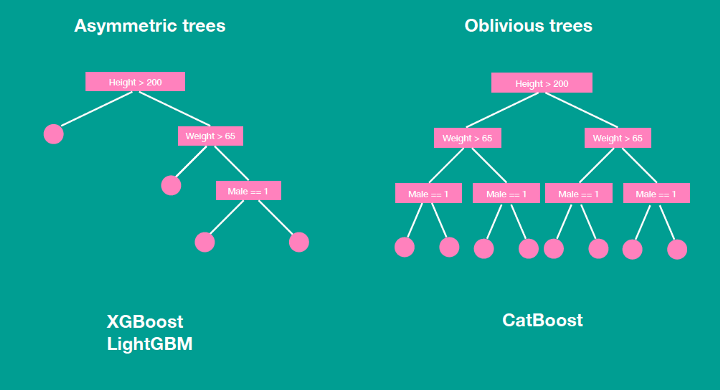
\includegraphics[scale=0.25]{DifBoost.png}
    \caption{Difference between CatBoost and XGBoost, \href{https://towardsdatascience.com/introduction-to-gradient-boosting-on-decision-trees-with-catboost-d511a9ccbd14}{(Source)}}
    \centering
\end{figure}

}





\section{Stacking}
%%%%%%%%%%%%%%%%%%%%%%%%%%%%%%%%%%%%%%%%%%%%%%%%%%%%%%%%%%%%%%%%%%%%%%%%%%%%%%%%%%%%%%%%%%%%%%%
\frame{\frametitle{Stacking}

\begin{itemize}
\item
\textbf{Blender} or \textbf{Meta-learner} or \textbf{Meta-classifier} takes predictions of each predictor as inputs and makes the final prediction. Basically we train a model to perform aggregation.

\begin{figure}[t]

    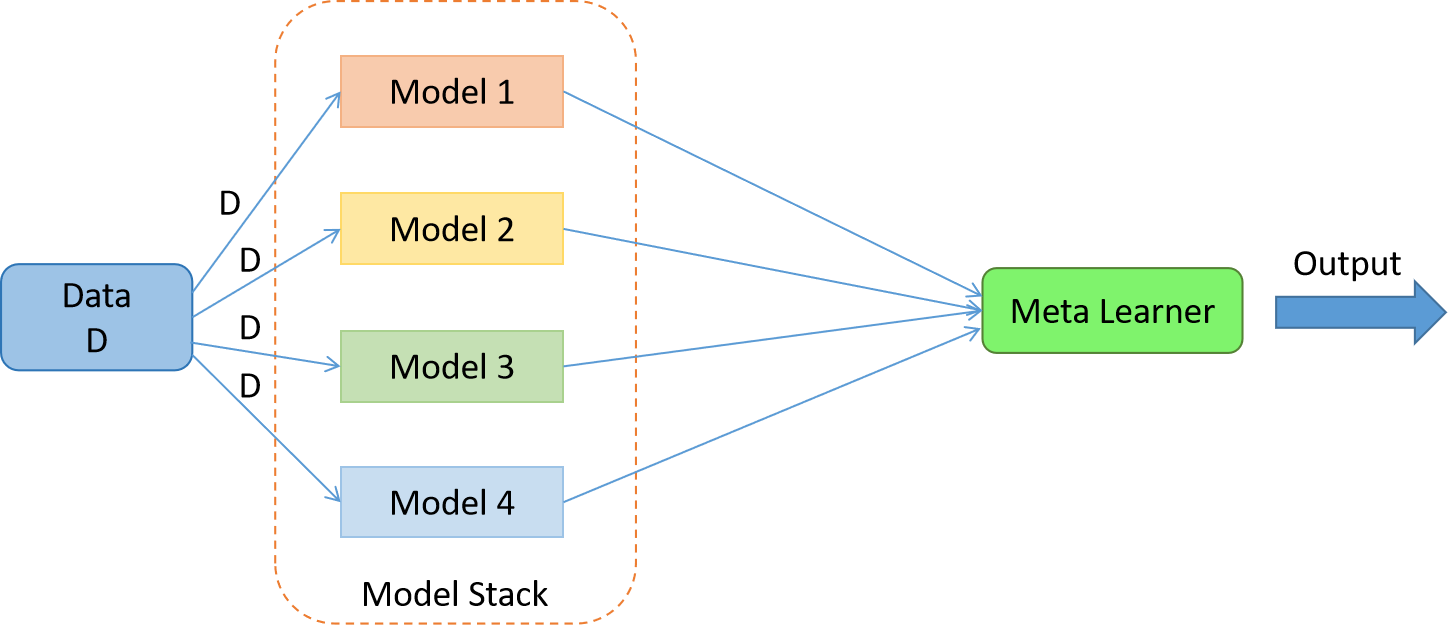
\includegraphics[scale=0.4]{Stacking.png}
    \caption{Example of Stacking, \href{https://www.analyticsvidhya.com/blog/2021/08/ensemble-stacking-for-machine-learning-and-deep-learning/}{(Source)}}
    \centering
\end{figure}
\end{itemize}
}
\frame{\frametitle{Features of Stacking}
\vspace{-3cm}
\begin{itemize}
\item
Usually has weak-learners of different types.
\item
Meta-learner tries to learn which weak-learner is more important.
\item
The weak-learners are trained in \textbf{parallel}, but the meta learner is trained \textbf{sequentially}. 
\item
Once the weak-learners are trained, their weights are kept static to train the meta-learner.
\item
Usually, the meta-learner is trained on a different subset than what was used to train the weak-learners.
\item
It is common to use a linear model for aggregation to avoid complexity.


\end{itemize}
}


\frame{\frametitle{Training Blender}
\vspace{-3cm}
\begin{itemize}
\item
To train the blender, a common approach is to use a \textbf{hold-out set}.
\item
First, the training set is split into two subsets. The first subset is used to train the predictors in the first layer.
\item
Next, the first layer’s predictors are used to make predictions on the second (held-out) set.
\item
Then we train the blender on this new training set, so it learns to predict the target value, given the first layer’s predictions.
% \begin{figure}[t]
%     \includegraphics[scale=0.4]{Holdout1.png}
%     \caption{Split training set into two subsets}
%     \centering
% \end{figure}
\end{itemize}
}

\frame{\frametitle{Training Blender}
% \begin{figure}[t]
%     \includegraphics[scale=0.2]{Holdout2.png}
%     \caption{Train, Predict,  Blend}
%     \centering
% \end{figure}

}


\frame{\frametitle{Stacking with Cross-Validation}
\begin{itemize}
\item
The problem with this method is that it has a high tendency to suffer from extensive overfitting. 
\item
A better alternative would be to use stacking with k-fold cross-validation or leave-one-out cross-validation.
\begin{figure}[t]
    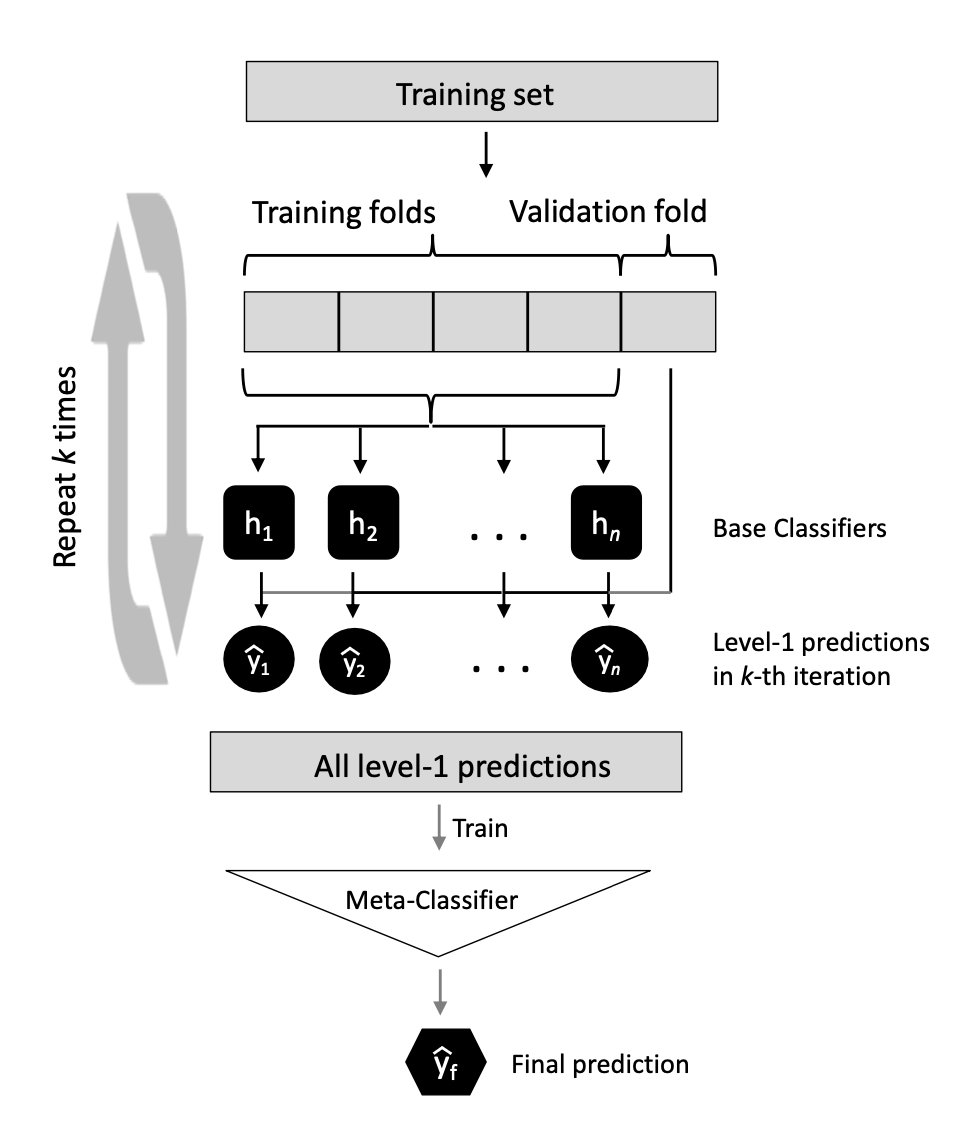
\includegraphics[scale=0.25]{StackCV.png}
    \caption{Example of Stacking with Cross-validation\cite{notes}}
    \centering
\end{figure}
\end{itemize}
}
% \frame{\frametitle{Multilayer Stacking}
% \begin{itemize}
% \item
% It is possible to train several different blenders, to get a whole layer of blenders.
%     \begin{itemize}
%     \item
%     Split the training set into three subsets
%     \item
%     The first one is used to train the first layer
%     \item
%     The second one is used to create the training set used to train the second layer (using predictions made by the predictors of the first layer)
%     \item
%     The third one is used to create the training set to train the third layer (using predictions made by the predictors of the second layer). 
%     \end{itemize}
% \item
% Once this is done, we can make a prediction for a new instance by going through each layer sequentially.
% \end{itemize}
% }


\frame{\frametitle{Multilayer Stacking}
% \begin{figure}[t]
%     \includegraphics[scale=0.4]{MulStack.png}
%     \caption{Multilayer Stacking}
%     \centering
% \end{figure}
}



\section{Conclusion}
%%%%%%%%%%%%%%%%%%%%%%%%%%%%%%%%%%%%%%%%%%%%%%%%%%%%%%%%%%%%%%%%%%%%%%%%%%%%%%%%%%%%%%%%%%%%%%%
\frame{\frametitle{Key Elements}
\vspace{-1cm}
\begin{itemize}
\item Bagging
    \begin{itemize}
    \item Bootstrap samples of the training dataset
    \item Unpruned decision trees fit on each sample
    \item Simple voting or averaging of predictions
    \end{itemize}
    
\item Stacking
    \begin{itemize}
    \item Unchanged training dataset
    \item Different machine learning algorithms for each ensemble member
    \item Machine learning model to learn how to best combine predictions
    \end{itemize}    

\item Boosting
    \begin{itemize}
    \item Bias training data toward those examples that are hard to predict
    \item Iteratively add ensemble members to correct predictions of prior models
    \item Combine predictions using a weighted average of models
    \end{itemize}
    
\end{itemize}
% \begin{figure}[t]
%     \includegraphics[scale=0.2]{Comparison.png}
%     \centering
% \end{figure}
}





%%%%%%%%%%%%%%%%%%%%%%%%%%%%%%%%%%%%%%%%%%%%%%%%%%%%%%%%%%%%%%%%%%%%%%%%%%%%%%%%%%%%%%%%%%%%%%%
\frame{\frametitle{Resources}
\printbibliography
%   \bibliographystyle{ieeetr}%{IEEEtrans}%{latex8}%
% 	\bibliography{references}
}




\frametitle{Final Notes}
\centering
\vspace{50 pt}
\textbf{Thank You!}
\vspace{50pt}

\textbf{Any Question?}
%%%%%%%%%%%%%%%%%%%%%%%%%%%%%%%%%%%%%%%%%%
\end{document}




% - https://towardsdatascience.com/what-are-ensemble-methods-in-machine-learning-cac1d17ed349
% - https://towardsdatascience.com/https-medium-com-vishalmorde-xgboost-algorithm-long-she-may-rein-edd9f99be63d
% - https://www.nvidia.com/en-us/glossary/data-science/xgboost/
% - https://towardsdatascience.com/a-beginners-guide-to-xgboost-87f5d4c30ed7
% - https://towardsdatascience.com/catboost-vs-light-gbm-vs-xgboost-5f93620723db
% - Hands-on machine learning Chapter 7
% - https://medium.com/@silvaan/ensemble-methods-bagging-and-pasting-in-scikit-learn-723f4183cdf4
% - https://machinelearningmastery.com/tour-of-ensemble-learning-algorithms/
% - https://www.analyticsvidhya.com/blog/2021/06/understanding-random-forest/
% - https://www.toptal.com/machine-learning/ensemble-methods-machine-learning#:~:text=Ensemble%20methods%20are%20techniques%20that,winning%20solutions%20used%20ensemble%20methods.
